%% V1.0
%% by Gabriel Garcia, gabrcg@gmail.com
%% This is a template for Udacity projects using IEEEtran.cls

%% Be Udacious!

\documentclass[10pt,journal,compsoc]{IEEEtran}

\usepackage[pdftex]{graphicx}    
\usepackage{cite}
\hyphenation{op-tical net-works semi-conduc-tor}


\begin{document}

\title{Where Am I?}

\author{Lucas Wohlhart}

\markboth{Localization project, Robotics Nanodegree Program, Udacity}%
{}
\IEEEtitleabstractindextext{%

\begin{abstract}
The goal of the project at hand is the examination of the capabilities of a widely used localization technique known as Adaptive Monte Carlo Localization (AMCL).
This method is based on a particle filter algorithm which will be conceptionally compared to another localization strategy using a Kalman Filter. 
For the evaluation of the localization method, two different robots models are placed in a ROS/Gazebo/RViz simulation environment in which they have to navigate through a maze world to reach a specified goal position.
These two mobile robots both feature a differential drive, one of which is given by the Udacity project description and the creation of the second (custom) robot model will be discussed within this report.
\end{abstract}

% Note that keywords are not normally used for peerreview papers.
\begin{IEEEkeywords}
Robot, IEEEtran, Udacity, \LaTeX, Localization.
\end{IEEEkeywords}}


\maketitle
\IEEEdisplaynontitleabstractindextext
\IEEEpeerreviewmaketitle
\section{Introduction}
\label{sec:introduction}

\IEEEPARstart{T}{he} capability of accurately determining the pose of a mobile robot is a crucial necessity for being able to autonomously navigate any given environment.
The problem of localization poses three challenges to tackle, which are known as: local localization, global localization and the kidnapped robot problem.
The goal of local localization is to keep track of the pose changes due to robot movement given a known initial pose. In global localization the robots pose starts out as being unknown and the objective is to determine the pose by comparing observations to a ground truth map. The kidnapped robot problem is similar to global localization since the goal is also to find the robots pose without knowing it's initial location, but with the challenging additional constraint that the robot might be randomly placed at an entirely different spot in the world at any time. 
This project tackles the problem of global localization which, if implemented and tuned correctly, enables the robots to autonomously navigate the maze world depicted in Figure~\ref{fig:maze} to reach a specified goal pose. 


%example for inserting image
\begin{figure}[thpb]
      \centering
      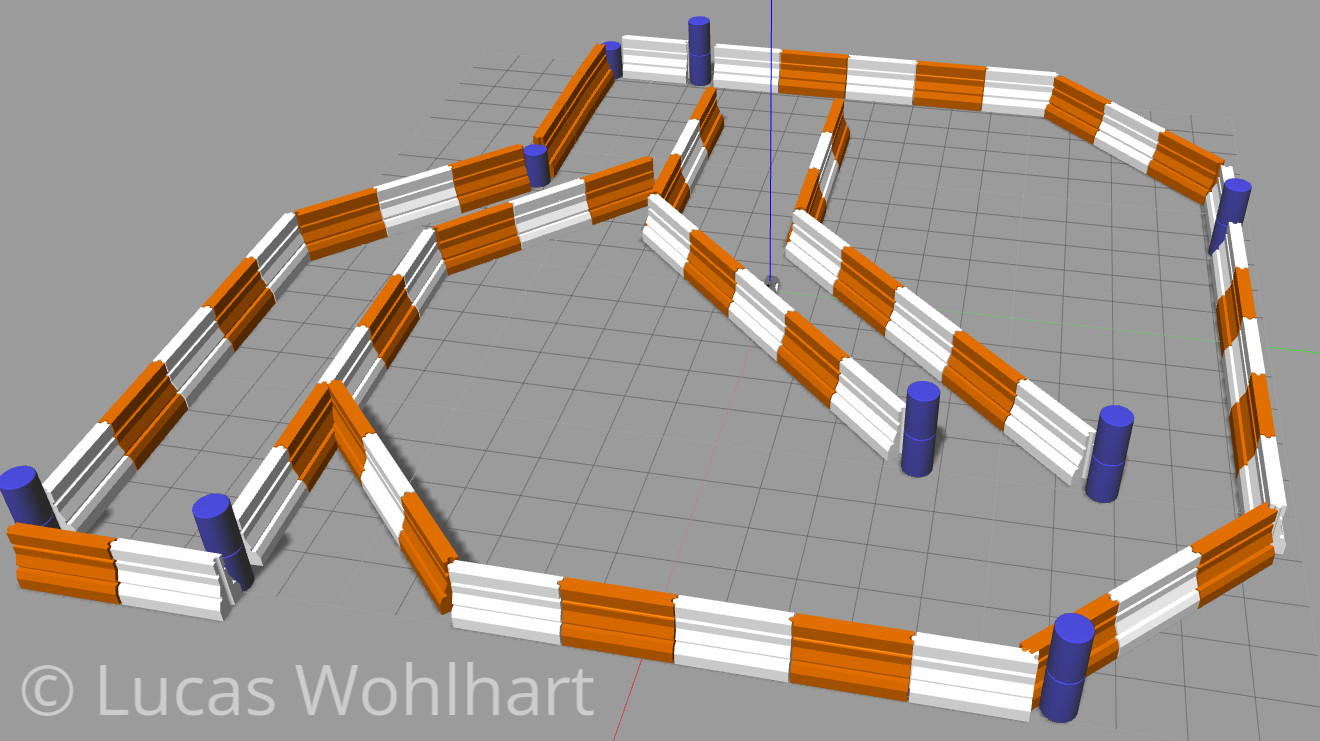
\includegraphics[width=\linewidth]{maze_world}
      \caption{Maze environment}
      \label{fig:maze}
\end{figure}


% %example for building table
% \begin{table}[h]
% \caption{Table}
% \label{table_example}
% \begin{center}
% \begin{tabular}{|c||c|}
% \hline
% One & Two\\
% \hline
% Three & Four\\
% \hline
% \end{tabular}
% \end{center}
% \end{table}



\section{Background}
Solving a localization problem boils down to modelling the robots pose changes resulting from the motions executed by the robot and interpreting the available sensor readings to gather evidence from the environment which can be compared to a known ground truth map.
Both these processes are subject to noise since motions can't be performed with absolute accuracy and sensors don't capture the exact truth about the world.

... EKF for local localization;
AMCL for global localization
choose AMCL; easier implementation; possible handling of kidnapped robot problem; simple modelling of nonlinear motions; initial state not necessarily known


\subsection{Kalman Filters}
The Kalman Filter is a widely used state estimation algorithm which starts out with an initial state (e.g. a state vector holding the estimated x and y position and the angular orientation of a robot) as well as a covariance matrix expressing the certainty of the estimate and iteratively applies measurement updates and state predictions for each motion step of the robot.

The state prediction step takes the current motion commands of the robot, maps them to the state domain using the predefined state transition matrix and combines the result with the prior state and covariance plus additional gaussian noise to account for noisy motions. This yields the posterior belief about the robots state after a motion step.

The measurement update step uses the measurement function to map the previously calculated posterior state of the prediction step to the measurement domain. This means calculating the expected values of all available sensors, assuming the robot were in this exact state. Computing the difference between this assumption and the actual sensor readings yields the measurement residual.
The so called Kalman Gain is then computed by projecting the covariance to the measurement domain, adding potential measurement noise to all components and reprojecting this result to the state domain. This is a measure indicating the ratio of preserving the previous state estimate and taking in the new measurement evidence. It ranges from a 0-vector which keeps the previous state estimate entirely, to the pseudo inverse of the measurement function which overrides the estimate with the incoming measurement data.

Therefore the Kalman Gain is subsequently used to update the state and covariance estimate.

One drawback of the standard Kalman Filter is that it can't deal with non linear state transitions or measurement functions. Applying a non linear transformation on a Gaussian distribution yields a probability distribution which is non Gaussian and since robots usually perform non linear motions such as driving along a circle or a curve the standard Kalman Filter is not usable for most robotics applications.
To overcome this problem the Extended Kalman Filter (EKF) was introduced which linearizes the non-linear transformations by approximating them with a first order Taylor series expansion. This linearization is only valid for a small region but if the update cycles are short enough the EKF has shown to be able to produce a good and stable state/pose estimation.


\subsection{Particle Filters}
A particle filter algorithm for robot localization starts by instantiating a number of particles each representing one guess about the position and orientation of the robot. For every particle a weight can be calculated which corresponds to the likelihood of observing the current readings from the available range-finder senors (e.g.  lidar, RGB-D cameras or others). If a particle matches the observation compared to the ground thruth deduced from the known map better, it gets a bigger weight than others which are less likely. Every motion step of the robot is also applied to each particle with some added noise. After a specific resample interval (usually also every motion step) the particles are then randomly resampled based on their weights and new particles might be spawned in proximity to the previously higher weighted particles. 

By iteratively applying the algorithm:
\begin{itemize}      
      \item motion update: apply robots motion with noise to each particle
      \item sensor update: assign weights to particles based likelihood of matching sensor readings
      \item resample: randomly sample current particle set and insert new particles based on weighted probabilities
\end{itemize}
the particles converge to the true pose of the robot because those which best fit the incoming evidence from the sensors have the highest chance of surviving the resample step.


\subsection{Comparison / Contrast}
Explain the benefits and disadvantages of using a Kalman Filter / Particle Filter. Why would you use one over the other? Also inform the reader that the work presented here will be using only particle filters. 

%example for Bullet point list
\begin{itemize}
\item example 1
\item example 2
\end {itemize}

%example for numbered list
\begin{enumerate}
\item example 1
\item example 2
\end{enumerate}

\section{Simulations}
This section should discuss the performance of robots in simulation. Items to include are the robot model design, packages used, and the parameters chosen for the robot to properly localize itself. The information provided here is critical if anyone would like to replicate your results. After all, the intent of reports such as these are to convey information and build upon ideas so you want to ensure others can validate your process.
You should have at least two images here: one that shows your standard robot used in the first part of the project, and a second robot that you modified / built that is different from the first robot. Remember to watermark all of your images as well. 

\subsection{Achievements}
You should describe what you achieved for localization in the project with the benchmark model and your own model. Includes charts and graphs show how parameters affect your performance. 

% Robot Models
\subsection{Benchmark Model}
\subsubsection{Model design}
The Robot's design considerations should include: the size of the robot, the layout of sensors. This information can be shown in the form of a chart / table.

\subsubsection{Packages Used}
The packages used in the project should be specified as well as the topics received and published; the services it used and provided should also be addressed. 

\subsubsection{Parameters}
Localization parameters in the AMCL node should be described, as well as move\_base parameters in the configuration file. You should be able to clearly demonstrate your understanding of the impact of these parameters.

\subsection{Personal Model}
% ditto
\subsubsection{Model design}
\subsubsection{Packages Used}
\subsubsection{Parameters}


\section{Results}
Present an unbiased view of your robot's performance and justify your stance with facts. Do the localization results look reasonable? What is the duration for the particle filters to converge? How long does it take for the robot to reach the goal? Does it follow a smooth path to the goal? Does it have unexpected behavior in the process? \\
For demonstrating your results, it is incredibly useful to have some watermarked charts, tables, and/or graphs for the reader to review. This makes ingesting the information quicker and easier.

\subsection{Localization Results}
\subsubsection{Benchmark}
\subsubsection{Student}

\subsection{Technical Comparison} % only facts
Discuss the difference of the layout, parameters, performance etc. between the benchmark robot and your robot. It is acceptable for your custom robot to perform worse than the provided robot. The focus is on learning and understanding, not performance. 

\section{Discussion}
This is the only section of the report where you may include your opinion. However, make sure your opinion is based on facts. If your robot performed poorly, make mention of what may be the underlying issues. If the robot runs well, which aspects contribute to that? Again, avoid writing in the first person (i.e. Do not use words like "I" or "me"). If you really find yourself struggling to avoid the word "I" or "me"; sometimes, this can be avoid with the use of the word “one”. As an example: instead of : "I think the robot cannot localize itself because the sensor does not provide enough information for localization" try: "one may believe the localization performance is poor because the sensor layout is not able to provide enough information for localization". They say the same thing, but the second avoids the first person. 

\subsection{Topics}
\begin{itemize}
\item Which robot performed better?
\item Why it performed better? (opinion)
\item How would you approach the 'Kidnapped Robot' problem?
\item What types of scenario could localization be performed?
\item Where would you use MCL/AMCL in an industry domain?
\end {itemize}

\section{Conclusion / Future work}
This section is intended to summarize your report. Your summary should include a recap of the results, did this project achieve what you attempted, how would you deploy it on hardware and how could this project be applied to commercial products? 
For Future Work, address areas of work that you may not have addressed in your report as possible next steps. This could be due to time constraints, lack of currently developed methods / technology, and areas of application outside of your current implementation. Again, avoid the use of the first-person.

\subsection{Modifications for Improvement}
Examples:
\begin{itemize}
\item Base Dimension
\item Sensor Location
\item Sensor Layout
\item Sensor Amount
\end{itemize}

\subsection{Hardware Deployment}
\begin{enumerate}
\item What would need to be done?
\item Computation time/resource considerations?
\end{enumerate}



\bibliography{bib}
\bibliographystyle{ieeetr}

\end{document}